\chapter{Grundlegendes}

MapReduce ist ein Programmiermodell, um große Datenmengen paralell (im normalfall in Clustern von Servern) zu analysieren und zu verarbeiten. Der Alogrithmus lässt sich in vier wesentliche Phasen einteilen, diese können anhand eines simplen Beispiels erklärt  werden.

\begin{figure}[!h]
	\centering
	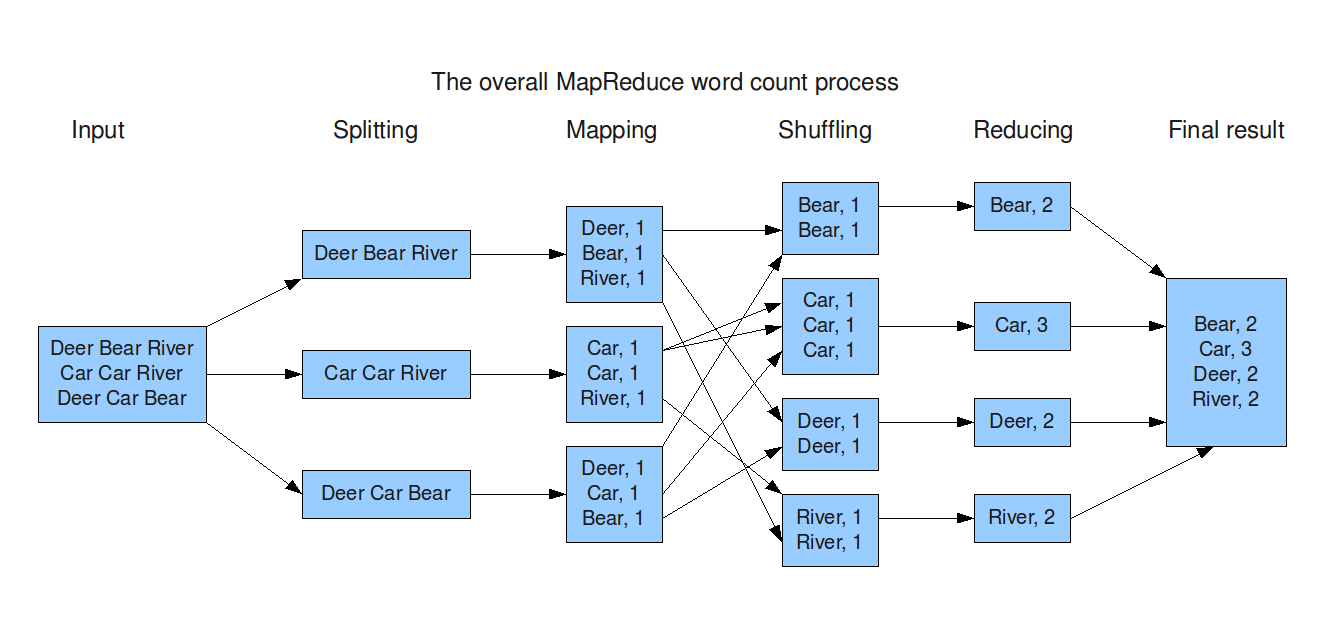
\includegraphics[width=\linewidth]{images/Phases.png}
	\caption{}
	\label{robotino_urdf}
\end{figure}

\section{Phase 1: Map}

x 